% ---
% CARACTERIZAÇÃO DA INTERNET DAS COISAS
%
% ---

\chapter{Caracterização da Internet das Coisas}

O primeiro passo para definir as ferramentas para o desenvolvimento de
\textit{software} para a \textit{Internet} das Coisas - \textit{Internet of Things} (\textit{IoT}) é entender a formação de
seus componentes e plataforma, empregadas para a Inteligência. Assim
visualizando a implementação em plataformas de desenvolvimento, como o
\textit{Raspberry PI B+}.

\section{Componentes}

A \textit{IoT} engloba os seguintes componentes: Interconexão,
Instrumentação e Inteligência, conforme a representação do conceito Planeta
Inteligente - \textit{Smarter Planet} da \textit{International Business
  Machines} (\textit{IBM}) na figura \ref{fig:pilares-da-iot}.

\begin{figure}[H]
    \centering
    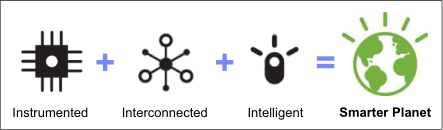
\includegraphics[width=0.7\linewidth]{figuras/pilares-da-iot}
    \caption{Os Três Pilares de um Planeta Inteligente}
    \label{fig:pilares-da-iot}
\end{figure}

A interconexão é construída pela conectividade com as redes locais e a
\textit{Internet} através de várias conexões física, tais como
\textit{Bluetooth}, \textit{Ethernet} e Fidelidade Sem Fio - \textit{Wireless
  Fidelity} (\textit{Wi-Fi}).

A instrumentação é construída pelos sensores e atuadores, no papel de
interfacear com o ambiente em indicar, monitorar e controlar os fenômenos de
diversas natureza. No processo de indicação estão os Diodos Emissores de Luz -
\textit{Light Emitting Diodes} (\textit{LEDs}) e os \textit{Displays}
Alfanumérico ou Gráfico. No processo de monitoração estão os sensores
eletrônicos para temperatura, umidade, presença, dentre outros... E no processo
de controle estão os motores e atuadores. Em uma constituição mais completa de
instrumentação estão a Identificação por Rádio Frequência -
\textit{Radio-Frequency IDentification} (\textit{RFID}), Sistema de
Posicionamento Global - \textit{Global Positioning System} (\textit{GPS}) e
Sistema de Navegação Inercial - \textit{Inertial Navigation System}
(\textit{INS}).

A inteligência é construída pelos algoritmos em \textit{software} embarcado, em
que realiza a junção do sistema computacional pelo processamento, análise e
ação da informação em conhecimento.

\section{Raspberry PI}

O \textit{Raspberry PI} é uma plataforma de desenvolvimento destinada para a
educação, desenvolvido por \textit{Even Upton} em 2006 da \textit{Raspberry PI
Foundation}. A figura \ref{fig:raspberrypi} apresenta a versão
\textit{Raspberry PI B+} utilizada no objeto de estudo, um sistema baseado em
\textit{Linux} utilizando a arquitetura de Máquina \textit{RISC} Avançada -
\textit{Advanced RISC Machine} \textit{ARM}) de baixo custo (por U\$ 40) do
tamanho de uma cartão de crédito.

\begin{figure}[H]
    \centering
    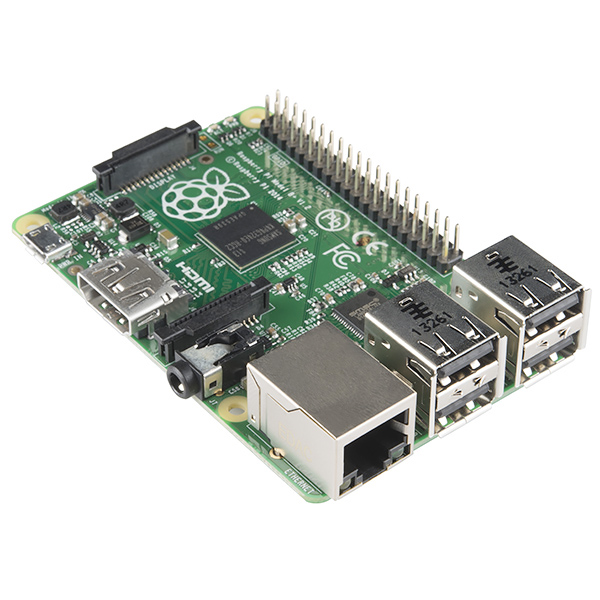
\includegraphics[width=10cm, height=10cm]{figuras/raspberrypi}
    \caption{Raspberry PI B+}
    \label{fig:raspberrypi}
\end{figure}

O ecossistema do \textit{Raspberry PI} possui uma grande comunidade na
\textit{WEB}, diversas opções de \textit{hardware} periféricos, variações de
sistema operacionais \textit{Linux} como especializações para Tempo Real -
\textit{Real Time} (\textit{RT}) e Computador com um Conjunto Reduzido de
Instruções - \textit{Reduced Instruction Set Computer} (\textit{RISC}).

Existem outros sistemas para uso na \textit{Internet} das Coisas, tais como
\textit{BeagleBone}, \textit{Cubieboard}, \textit{Odroid} dentre outros... A
maioria baseada no mesmo sistema computacional do \textit{Raspberry PI}, com
sistema \textit{Linux} em arquitetura \textit{ARM}.
